\section{Results}
\label{sec:results}

We calibrate the model using publicly available data on Strategy (MSTR), Bitcoin, and the company's balance sheet through December 1, 2025. This section reports the estimated parameters, computed indicators, and their economic interpretation. All figures referenced below are produced by the calibration pipeline and are included in the appendix.

\subsection{Calibrated Parameters}

Table~\ref{tab:params} reports the full set of estimated parameters.

\begin{table}[H]
\centering
\caption{Calibrated Model Parameters (as of December 1, 2025)}
\label{tab:params}
\begin{tabular}{@{}llrl@{}}
\toprule
\textbf{Parameter} & \textbf{Symbol} & \textbf{Value} & \textbf{Description} \\
\midrule
\multicolumn{4}{l}{\textit{BTC Price Dynamics}} \\
BTC drift & $\mu_S$ & 0.140 & Annualized historical return \\
BTC volatility & $\sigma_S$ & 0.488 & Annualized historical volatility \\
\midrule
\multicolumn{4}{l}{\textit{Premium OU Process}} \\
Mean-reversion speed & $\kappa$ & 4.081 & Annual rate of reversion to $\theta$ \\
Long-run mean & $\theta$ & 0.705 & Corresponds to a $\approx 2.0\times$ NAV premium \\
Premium volatility & $\sigma_\pi$ & 1.417 & Annualized diffusive vol of log-premium \\
BTC--premium correlation & $\rho$ & $-0.491$ & Negative: premium compresses on BTC rallies \\
Premium--BTC sensitivity & $\gamma_{\pi S}$ & $-1.480$ & Regression coefficient \\
\midrule
\multicolumn{4}{l}{\textit{Holdings Dynamics}} \\
Continuous drift & $\alpha$ & 0.000 & Not significantly different from zero \\
Jump intensity & $\lambda_M$ & 17.295 & $\approx$17.3 financing events per year \\
Mean jump size & $\mathbb{E}[\Delta H]$ & 6{,}887 & BTC per event \\
\midrule
\multicolumn{4}{l}{\textit{Balance Sheet (Initial Conditions)}} \\
BTC price & $S_0$ & \$86{,}286 & \\
BTC holdings & $H_0$ & 649{,}870 & \\
Outstanding debt & $D_0$ & \$8.22B & Face value \\
Shares outstanding & $N_0^{\text{sh}}$ & 267.7M & \\
Current log-premium & $\pi_0$ & $-0.042$ & Slightly below NAV \\
\bottomrule
\end{tabular}
\end{table}

\paragraph{BTC dynamics.} The estimated BTC annualized volatility of 48.8\% is consistent with the cryptocurrency's historical behavior over the sample period. The positive drift of 14.0\% reflects the secular upward trend in BTC price under the physical measure.

\paragraph{Premium process.} The OU parameters reveal fast mean-reversion ($\kappa = 4.08$, implying a half-life of approximately $\ln 2 / \kappa \approx 62$ calendar days) toward a long-run log-premium of $\theta = 0.705$, corresponding to equity trading at roughly $2.0\times$ NAV in the long run. The premium volatility is high ($\sigma_\pi = 1.42$), reflecting the large swings in market sentiment around BTC treasury vehicles.

The estimated correlation $\rho = -0.49$ is economically significant and negative: when BTC price rises, the premium tends to compress, and vice versa. This suggests that BTC rallies are partially ``priced in'' through NAV increases, reducing the sentiment component. The regression coefficient $\gamma_{\pi S} = -1.48$ confirms this quantitatively---a 1\% BTC increase is associated with a 1.48 percentage point decrease in the log-premium, on average.

\paragraph{Holdings dynamics.} The continuous accumulation drift $\alpha$ is estimated at zero, indicating that all meaningful BTC acquisition occurs through discrete financing events rather than continuous purchasing. The jump intensity $\lambda_M = 17.3$ events per year implies roughly one financing event every three weeks on average. The mean purchase size of 6{,}887 BTC per event, at late-2025 prices, corresponds to approximately \$594 million per event---consistent with the scale of Strategy's ATM and convertible offerings.

\subsection{Computed Indicators}

Table~\ref{tab:indicators} summarizes the five diagnostic indicators.

\begin{table}[H]
\centering
\caption{Model-Implied Indicators (as of December 1, 2025)}
\label{tab:indicators}
\begin{tabular}{@{}lrl@{}}
\toprule
\textbf{Indicator} & \textbf{Value} & \textbf{Interpretation} \\
\midrule
IBGR (total) & 18.3\% & Annualized BTC accumulation rate \\
IBGR (per-share, 3yr) & 18.4\% & Annualized BTC-per-share growth \\
ILE & 1.172 & Structural leverage elasticity \\
TEE & $-0.308$ & Total equity--BTC elasticity \\
PMRI & $-1.506$ & Std.~devs below long-run mean premium \\
IFRD (mean, 3yr) & \$38.3B & Expected cumulative funding need \\
IFRD (95th pctl, 3yr) & \$80.3B & Tail funding need \\
Survival prob (3yr, $\varepsilon=0$) & 99.42\% & No-distress probability \\
Survival prob (3yr, $\varepsilon=10\%$) & 99.32\% & With 10\% buffer \\
\bottomrule
\end{tabular}
\end{table}

\subsubsection{IBGR: Implied BTC Growth Rate}

The model implies a total BTC accumulation rate of 18.3\% annually, driven entirely by discrete financing events (since $\alpha = 0$). Strikingly, the per-share IBGR of 18.4\% is nearly identical, indicating that share dilution from equity issuance has been almost perfectly offset by the volume of BTC acquired---the flywheel has been \emph{highly accretive} on a per-share basis.

This finding has direct implications for valuation: if the market expects the flywheel to continue operating at this pace, the premium over NAV reflects an expectation of compounding BTC-per-share growth at approximately 18\% annually, in addition to any appreciation in BTC itself.

\subsubsection{ILE: Implied Leverage Elasticity}

The ILE of 1.172 indicates moderate structural leverage. Strategy's BTC assets of approximately \$56.1 billion exceed its \$8.2 billion debt by a factor of 6.8, producing a leverage elasticity only modestly above 1.0. This means that, holding the premium fixed, a 10\% BTC decline would produce approximately an 11.7\% equity decline---manageable leverage that reflects the large cushion between assets and debt.

Figure~\ref{fig:ile_tee} (see results/figures/ile\_tee\_timeseries.png) shows the time series of ILE, which has declined from significantly higher levels in 2021--2022 when BTC prices were lower relative to debt, to its current low level as BTC appreciation has dwarfed the debt stack.

\subsubsection{TEE: Total Equity Elasticity}

The TEE of $-0.308$ presents a striking contrast to the ILE. While the balance-sheet leverage contributes positively (+1.172), the premium's negative sensitivity to BTC ($\gamma_{\pi S} = -1.48$) more than offsets it. The net effect is that, empirically, MSTR equity has moved \emph{inversely} to BTC on average in recent data---a counterintuitive result driven by the premium dynamics.

This decomposition is the TEE's primary analytical value: it separates the ``structural'' BTC exposure (ILE, which is always $\ge 1$) from the ``sentiment'' exposure ($\gamma_{\pi S}$, which can be any sign), revealing that short-term MSTR returns are dominated by premium fluctuations rather than BTC fundamentals.

\subsubsection{PMRI: Premium Mean-Reversion Index}

The PMRI of $-1.51$ indicates that the current premium ($\pi_0 = -0.042$, i.e., equity trading approximately at NAV) is 1.5 stationary standard deviations below the long-run mean ($\theta = 0.705$, i.e., $\approx 2\times$ NAV). Under the OU dynamics, this represents a mean-reverting opportunity: the model expects the premium to drift upward toward its long-run level with a half-life of roughly 62 trading days.

Figure~\ref{fig:premium} (see results/figures/premium\_timeseries.png) displays the premium time series, illustrating the mean-reverting behavior and the current below-average level.

\subsubsection{IFRD: Implied Funding Requirement}

The IFRD indicates that sustaining the model-implied BTC accumulation trajectory over three years requires, in expectation, approximately \$38.3 billion in financing, with a 95th percentile tail of \$80.3 billion. These are large numbers in absolute terms, but Strategy has demonstrated the capacity to raise capital at this scale through its ATM program and convertible issuances (the 21/21 plan alone targeted \$42 billion in financing).

Figure~\ref{fig:ifrd} (see results/figures/ifrd\_histogram.png) shows the simulated IFRD distribution, which is right-skewed, reflecting the positive correlation between BTC price and funding costs (higher BTC prices make each unit of BTC more expensive to acquire).

\subsubsection{Survival Probability}

The three-year survival probability of 99.42\% (99.32\% with a 10\% buffer) indicates that the current capital structure is highly resilient to distress. The large gap between BTC asset value (\$56.1B) and debt (\$8.2B) means that BTC would need to decline by approximately 85\% before assets breach the debt boundary---an extreme but not unprecedented scenario for cryptocurrency. The survival analysis incorporates the full joint dynamics, including the possibility of further BTC accumulation via the flywheel, which acts as a partial buffer (acquiring BTC at lower prices when the premium permits).

Figure~\ref{fig:assets} (see results/figures/assets\_debt\_nav.png) illustrates the historical evolution of assets, debt, and NAV, showing the growing cushion over time.

\begin{figure}[H]
\centering
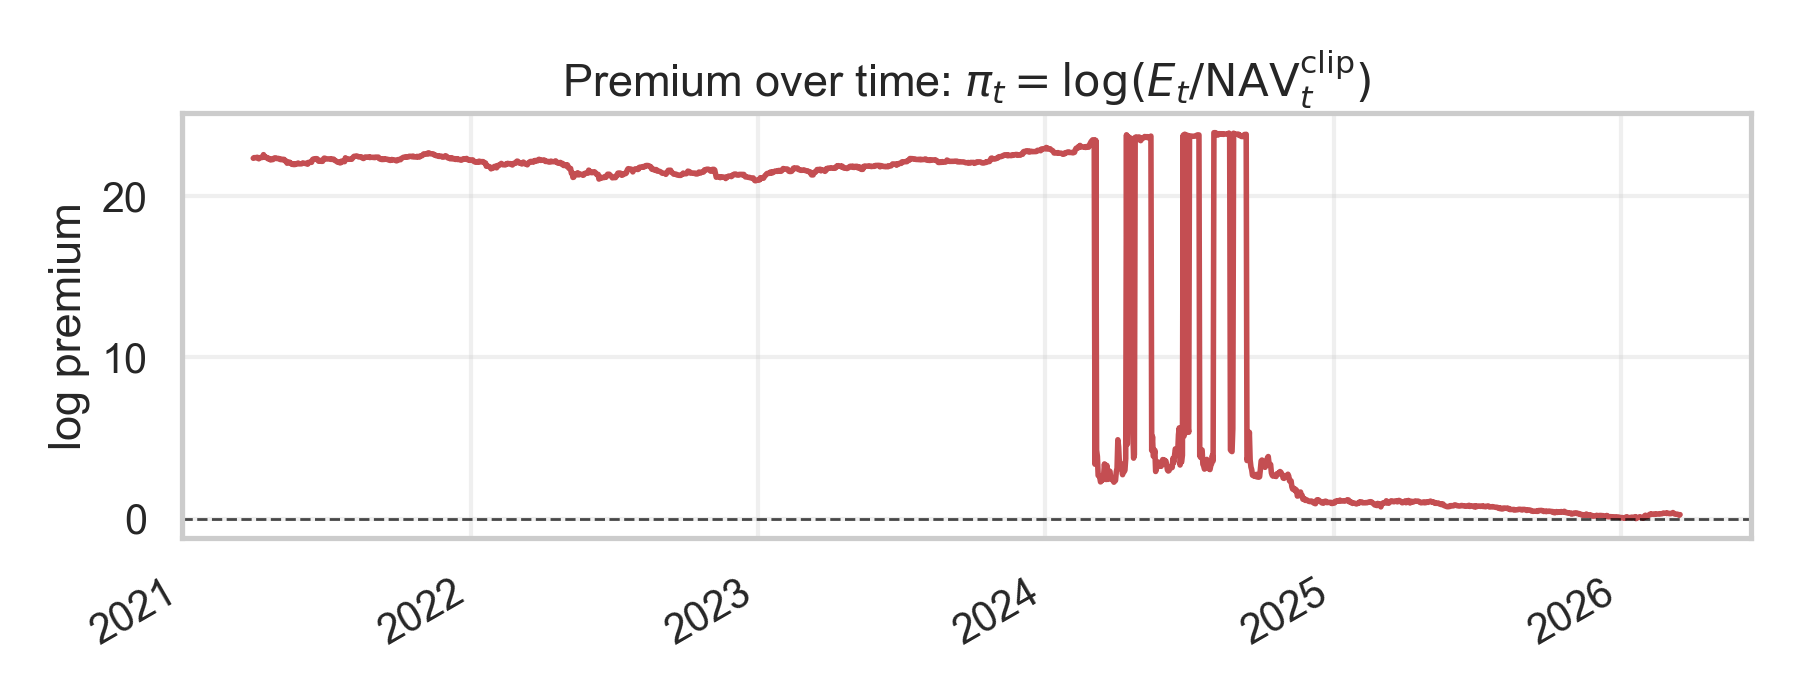
\includegraphics[width=0.85\textwidth]{../results/figures/premium_timeseries.png}
\caption{Historical log-premium $\pi_t = \log(E_t / \text{NAV}_t^{\text{clip}})$. The dashed line indicates the OU long-run mean $\theta = 0.705$. The premium exhibits clear mean-reverting behavior around this level.}
\label{fig:premium}
\end{figure}

\begin{figure}[H]
\centering
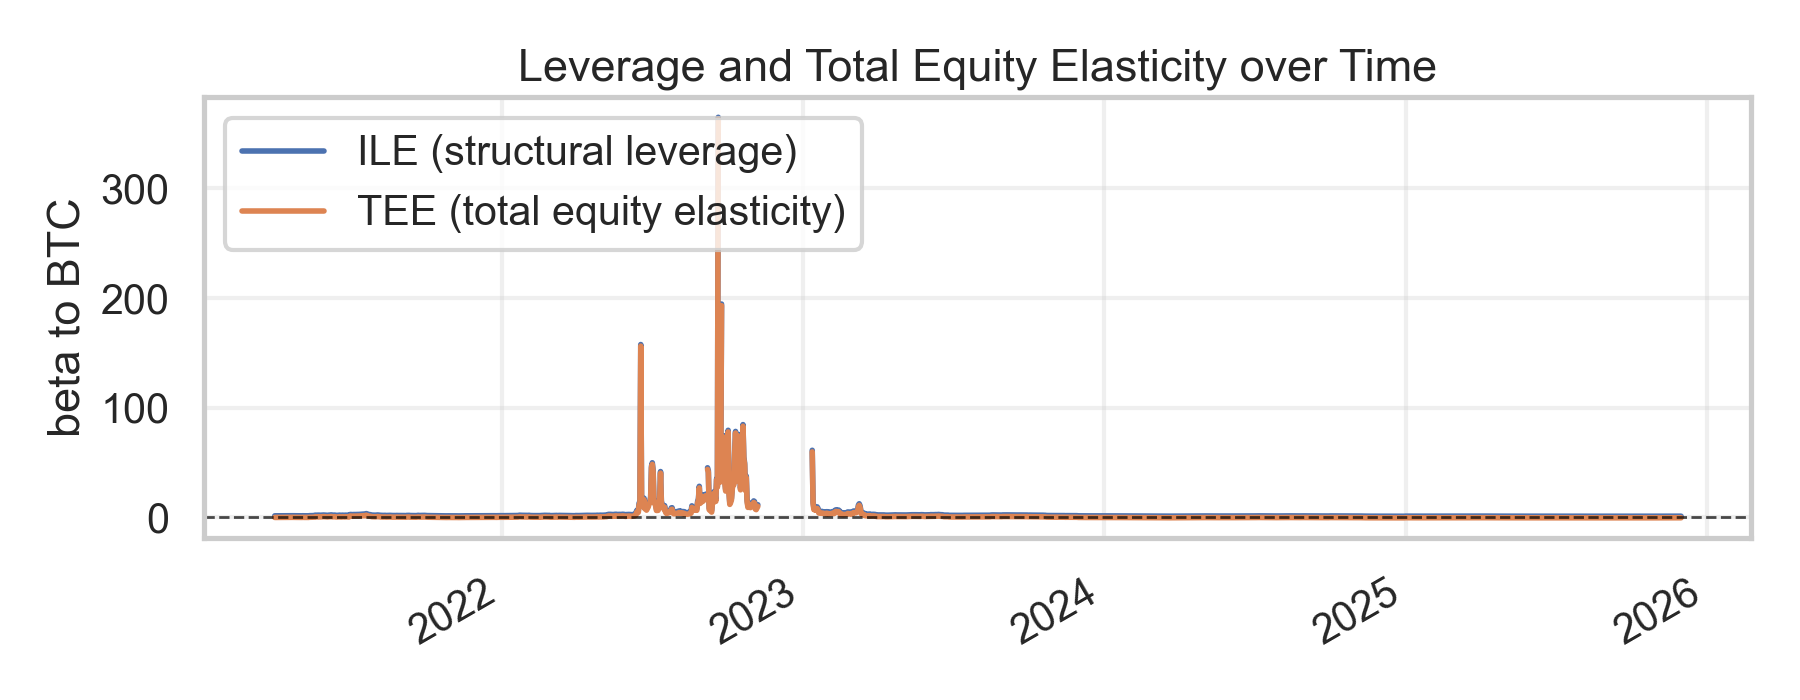
\includegraphics[width=0.85\textwidth]{../results/figures/ile_tee_timeseries.png}
\caption{Time series of Implied Leverage Elasticity (ILE) and Total Equity Elasticity (TEE). ILE has declined as BTC appreciation outpaced debt growth. TEE reflects the net of ILE and the negative premium--BTC sensitivity.}
\label{fig:ile_tee}
\end{figure}

\begin{figure}[H]
\centering
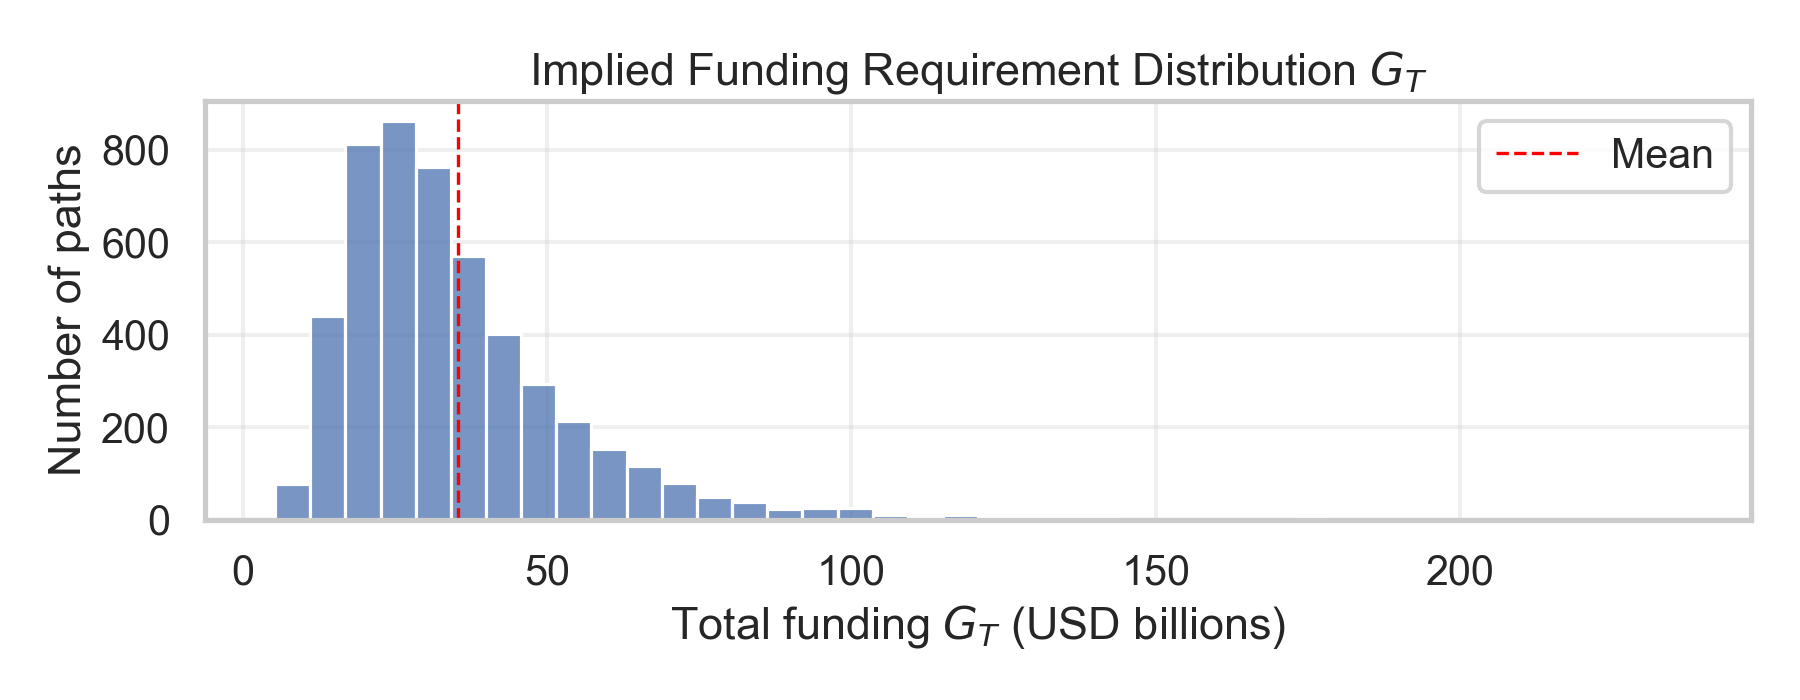
\includegraphics[width=0.85\textwidth]{../results/figures/ifrd_histogram.png}
\caption{Simulated three-year Implied Funding Requirement Distribution (IFRD). The distribution is right-skewed, with mean \$38.3B and 95th percentile \$80.3B.}
\label{fig:ifrd}
\end{figure}

\begin{figure}[H]
\centering
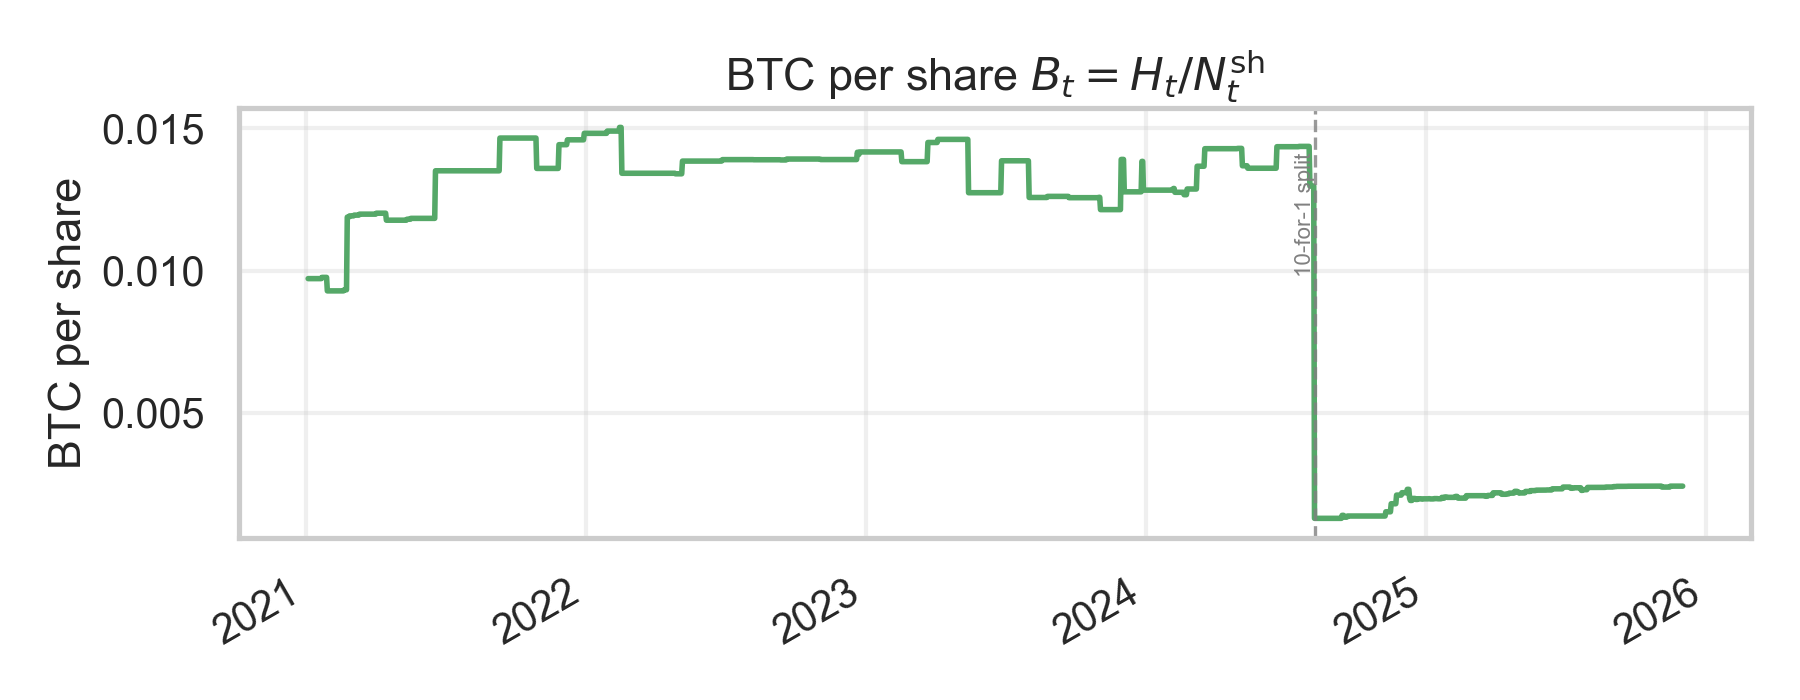
\includegraphics[width=0.85\textwidth]{../results/figures/btc_per_share_timeseries.png}
\caption{BTC per share ($B_t = H_t / N_t^{\text{sh}}$) over time. The upward trend confirms that Strategy's flywheel has been accretive despite significant share dilution.}
\label{fig:btc_per_share}
\end{figure}

\begin{figure}[H]
\centering
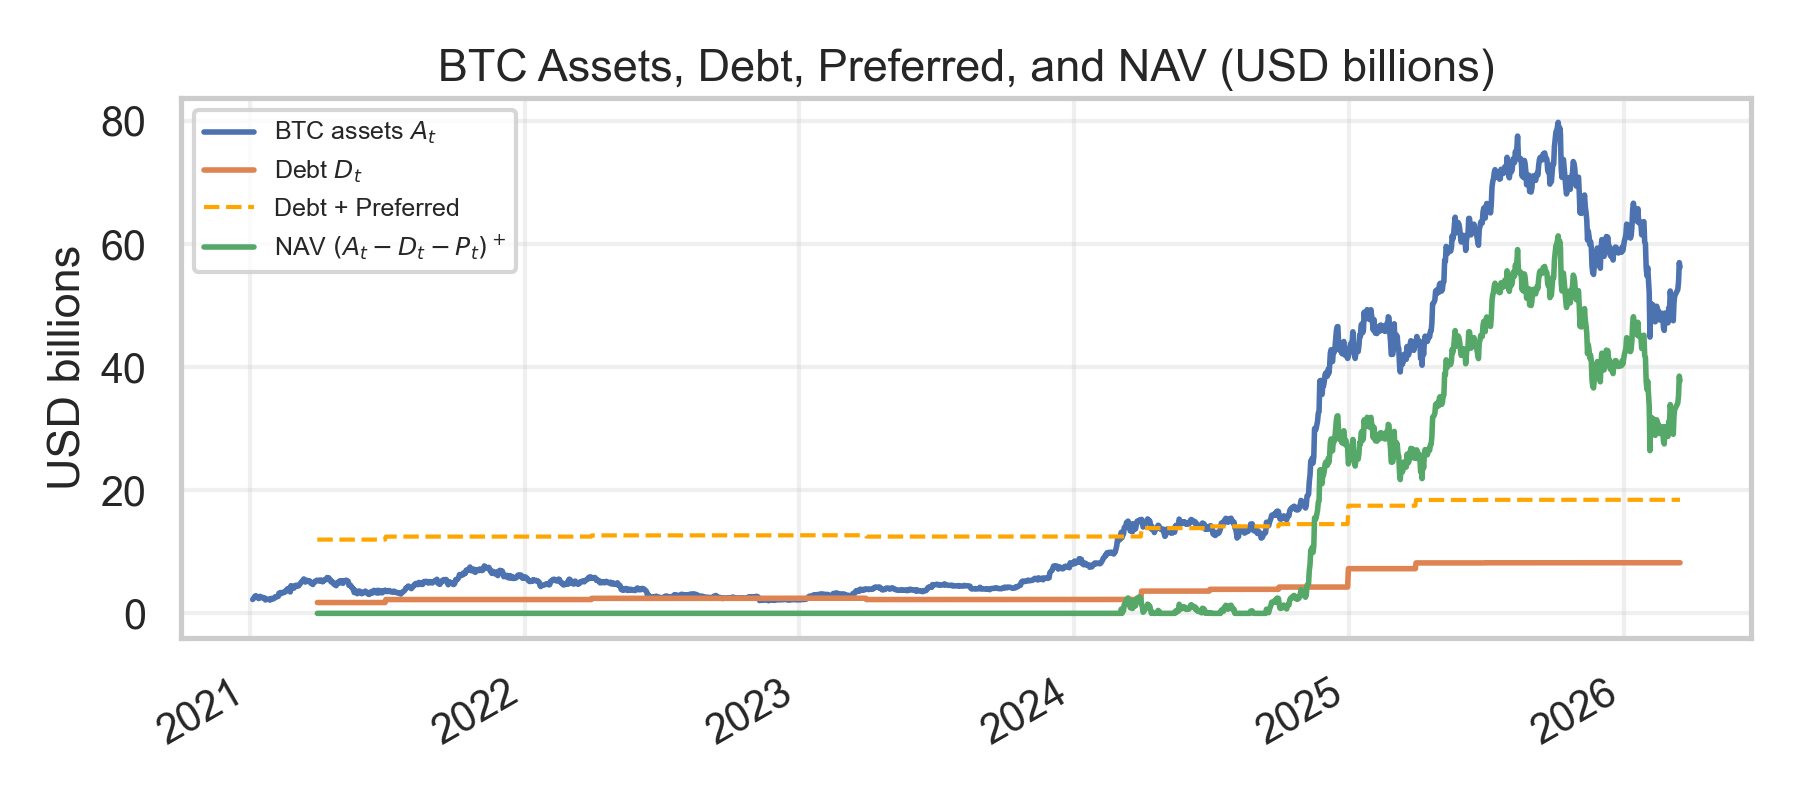
\includegraphics[width=0.85\textwidth]{../results/figures/assets_debt_nav.png}
\caption{BTC asset value ($A_t = H_t S_t$), outstanding debt ($D_t$), and NAV ($(A_t - D_t)^+$). The growing gap between assets and debt underpins the high survival probability.}
\label{fig:assets}
\end{figure}
